\documentclass[10pt]{article}

\usepackage[utf8]{inputenc}
\usepackage[french]{babel}
\usepackage[rigidchapters]{titlesec}
\usepackage{comment,fullpage}
\usepackage{hyperref}
\usepackage{comment,times,fancyvrb,amsmath,amsthm,amssymb,latexsym,xspace}
\usepackage{graphicx}
\usepackage{palatino}

\usepackage{minted}

\graphicspath{./Fig}

% Palatino for rm and math | Helvetica for ss | Courier for tt
\usepackage{mathpazo} % math & rm
\linespread{1.05}        % Palatino needs more leading (space between lines)
\usepackage[scaled]{helvet} % ss
\usepackage{courier} % tt
\normalfont

\usepackage[T1]{fontenc}
%\usepackage{listings}
\usepackage{color}
\usepackage{lastpage}
\usepackage{verbatim}
%\usepackage{enumitem}
 
\newenvironment{solution}{~\linebreak%
\textcolor{red}{\textsc{Correction}}\linebreak{\color{red}\rule{\textwidth}{0.7pt}}\medskip%
}{}
%{\hfill~\linebreak{\color{red}\rule{\textwidth}{0.7pt}}}

\excludecomment{solution}

%\setenumerate[0]{font=\itshape, label*=\thesection.\arabic*}


% Paramètres indiquant le titre de l'exam, et le fichier 
\providecommand{\titre}{Titre diapos}% fallback definition
\providecommand{\inputFile}{}% fallback definition

\begin{document}

\begin{center}
{\Large Test connaissances bases de données}\\\vspace{1ex}
\end{center}


\begin{center}
  \begin{figure}[htb]  
   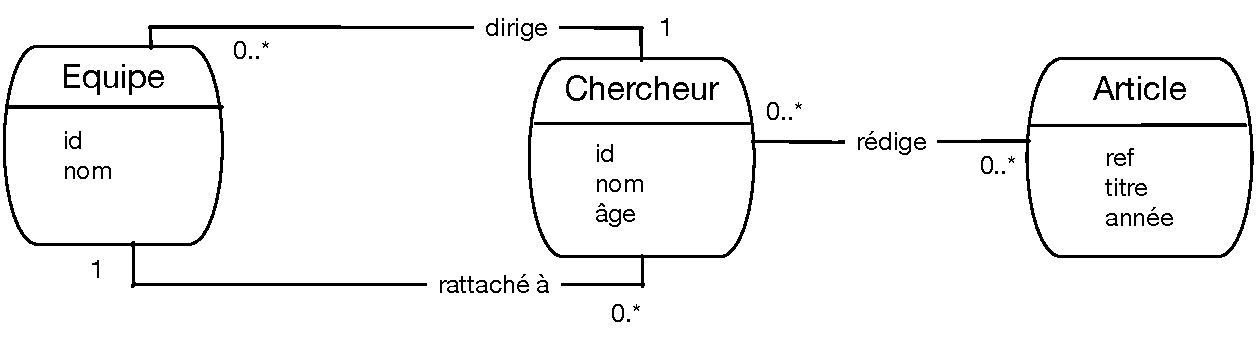
\includegraphics[scale=0.6]{exam-19-labo}
    \caption{Un laboratoire d'informatique}  
    \label{labo}  
  \end{figure}  
\end{center}


\section{Conception}

On modélise un laboratoire d'informatique afin de pouvoir gérer 
ses équipes, ses chercheurs et leurs publications (articles).
L'analyse donne le schéma  entité/association de la figure~\ref{labo}. 

\begin{enumerate}
 
   \item  Donnez les commandes {\tt CREATE TABLE} pour les tables de cette base, 
       avec les clés primaires et étrangères soigneusement indiquées
   
    \item On veut ajouter la position d'un chercheur dans l'ordre des auteurs pour un article. Où
        ajouter cette information, dans le modèle entité association et dans le modèle relationnel\,?
  \end{enumerate}
 
 
\section{SQL}

 Donnez les requêtes SQL suivantes:
 \begin{enumerate}

 \item Titre des articles parus depuis 2015 dont l'un au moins des auteurs appartient à l'équipe ``ROC''
\item Quels articles n'ont pas d'auteur\,?
 \item  Titre des articles parus depuis 2015 dont tous les auteurs appartiennent à l'équipe ``ROC'' 
 \item Nom des chercheurs qui dirigent une équipe à laquelle ils n'appartiennent pas
 \item Nom des chercheurs qui dirigent plus d'une équipe.
\end{enumerate}

\section{Les index}

J'ai un arbre B dont chaque bloc contient au moins 5 et au plus 10 entrées.
Quel est le nombre d’enregistrements que je peux indexer avec un arbre à 2 niveaux?
Expliquez le raisonnement.

\begin{enumerate}
 \item 20 au mieux, 10 au pire
 \item 100 au mieux, 50 au pire
 \item 100 au mieux, 25 au pire
 \item 200 au mieux, 100 au pire
\end{enumerate}


\section{Algorithmes}

Essayez de décrire l'algorithme de jointure par hachage dans un système relationnel.

\section{Transactions}

Expliquez la notion d'atomicité d'une transaction. Pourquoi est-ce important\,?

\medskip

Je suppose deux transactions concurrentes  $T_1$ et  $T_2$. Quelle(s) affirmation(s), parmi les suivantes, est (sont) vraie(s) 
dans un système transactionnel assurant les propriétés ACID\,?

\begin{enumerate}
   \item  Si $T_2$  débute après $T_1$,
       $T_1$  ne voit jamais les  mises à jour de $T_2$.
   
   \item $T_1$  ne voit pas ses propres mises à jour tant qu'elle n'a pas validé.
   
  \item Si $T_2$  débute après $T_1$,
       $T_1$  ne voit les  mises à jour de $T_2$ qu'après  que $T_2$ a effectué un \texttt{commit}.

  \item Si  $T_1$  et $T_2$  veulent modifier le même nuplet,
       cela déclenche un interblocage (\texttt{deadlock}).
   
\end{enumerate}

\end{document}
